\chapter{周期场中的电子态\label{ch:7}}

\noindent \textbf{1.\quad} 一维周期场中电子的波函数 $\psi_k(x)$ 应满足布洛赫定理。若晶体常数是 $a$,电子的波函数为

\begin{align*}
    (1) \quad & \Psi_k(x) = \sin \frac{\pi}{a}x \\
    (2) \quad & \Psi_k(x) = i \cos \frac{3\pi}{a}x \\
    (3) \quad & \Psi_k(x) = \sum_{l=-\infty}^{\infty} f(x-la)
\end{align*}

试求电子在这些状态的波矢。

\noindent \textbf{解:}

\begin{equation*}
    T_l \Psi = e^{i \vec{k} \cdot \vec{R}_l} \Psi
\end{equation*}

\begin{equation*}
    (1) \quad \Psi_k(x+a) = \sin \frac{\pi}{a} (x+a) = e^{i\pi} \Psi_k(x) = e^{ika} \Psi_k (x)
\end{equation*}

\begin{equation*}
    \therefore ka = \pi, \quad k = \frac{\pi}{a}
\end{equation*}

\begin{equation*}
    (2) \quad \Psi_k(x+a) = i\cos \frac{3\pi}{a} (x+a) = e^{i\pi} \Psi_k(x) = e^{ika} \Psi_k (x)
\end{equation*}

\begin{equation*}
    \therefore ka = \pi, \quad k = \frac{\pi}{a}
\end{equation*}

\begin{equation*}
    (3) \quad \Psi_k(x+a) = \sum_{l=-\infty}^{\infty} f(x+a-la) = \sum_{l=-\infty}^{\infty} f[x-(l-1)a] = \sum_{l=-\infty}^{\infty} f(x-la) \Psi_k (x)
\end{equation*}

\begin{equation*}
    \therefore ka = 0, \quad k = 0
\end{equation*}

\noindent \textbf{2.\quad} 电子在周期场中的势能

\begin{equation*}
    V(x) =
    \begin{cases}
        \frac{1}{2} m \omega^2 \left[b^2-(x-na)^2\right] & na-b \le x \le na+b \\
        0 & (n-1)a+b \le x \le na-b
    \end{cases}
\end{equation*}

且 $a=4b$,$\omega$ 是常数。试画出此势能曲线,并求此势能的平均值。

\noindent \textbf{解:}

势能曲线为:

\begin{equation*}
    \overline{V} = \frac{1}{a} \int_{-\frac{a}{4}}^{\frac{a}{4}} V(x) \dif x = \frac{1}{a} \int_{-\frac{a}{4}}^{\frac{a}{4}} \frac{1}{2} m \omega^2 \left[b^2 - (x-na)^2\right] \dif x = \frac{m \omega^2 a^2}{96}
\end{equation*}

\noindent \textbf{3.\quad} 用近自由电子模型处理上题,并求此晶体的第一个以及第二个禁带宽度。

\noindent \textbf{解:}

\begin{equation*}
    V(x) = \sum_n V_n e^{in \frac{2\pi}{a} x} = V_0 + \sum_{n \ne 0} V_n e^{in \frac{2\pi}{a} x}
\end{equation*}

为简单计算,令 $V_0=0$

\begin{align*}
    V_1 = \frac{1}{a} \int_{-\frac{a}{2}}^{\frac{a}{2}} V(x) e^{-i \frac{2\pi}{a} x} \dif x = \frac{m \omega^2 a^2}{4 \pi^2} \\
    V_2 = \frac{1}{a} \int_{-\frac{a}{2}}^{\frac{a}{2}} V(x) e^{-i \frac{4\pi}{a} x} \dif x = \frac{m \omega^2 a^2}{32 \pi^2}
\end{align*}

计算表明,第一个禁带宽度为:

\begin{equation*}
    2|V_1| = \frac{m \omega^2 a^2}{2\pi^2}
\end{equation*}

第二个禁带宽度为:

\begin{equation*}
    2|V_2| = \frac{m \omega^2 a^2}{16\pi^2}
\end{equation*}

\noindent \textbf{4.\quad} 已知一维晶体的电子能带可写成

\begin{equation*}
    E(k) = \frac{\hbar^2}{m a^2} \left(\frac{7}{8}-\cos ka + \frac{1}{8} \cos 2ka\right)
\end{equation*}

式中 $a$ 是晶格常数。试求:

\begin{enumerate}
    \item 能带的宽度;
    \item 电子在波矢 $k$ 的状态时的速度;
    \item 能带底部和顶部电子的有效质量。
\end{enumerate}

\noindent \textbf{解:}

\begin{enumerate}
    \item 分析能量的表达式
        \begin{align*}
            E(k) &= \frac{\hbar^2}{m a^2} \left(\frac{7}{8}-\cos{ka} + \frac{1}{8} \cos 2ka\right) \\
            &= \frac{\hbar^2}{m a^2} \left[\frac{1}{4} \left(\cos{ka}-2\right)^2 - \frac{1}{4}\right] \\
        \end{align*}
        当 $k=0$ 时,$E_{min}=0$;当 $k=\frac{\pi}{a}$ 时,$E_{max}=\frac{2\hbar^2}{m a^2}$。所以能带的宽度为
        \begin{equation*}
            \Delta E = E_{max} - E_{min} = \frac{2\hbar^2}{m a^2}
        \end{equation*}
    \item 电子的速度为
        \begin{align*}
            \vec{v} &= \frac{1}{\hbar} \Delta_k E(\vec{k}) \\
            &= -\frac{\hbar}{4ma} (\sin{2ka} - 4 \sin{ka})
        \end{align*}
    \item 能带底部,将 $E(k)$ 在 $k=0$ 附近用泰勒展开,可得
        \begin{equation*}
            E = E_{min} + \frac{\hbar^2 k^2}{4m} = E_{min} + \frac{\hbar^2 k^2}{2 m^*}
        \end{equation*}
        比较可得
        \begin{equation*}
            m^* = 2m
        \end{equation*}
        同理,在能带顶部,将 $E(k)$ 在 $k=\frac{\pi}{a}$ 附近用泰勒展开,令 $k=\frac{\pi}{a}+\delta k$,可得
        \begin{equation*}
            E = E_{max} - \frac{3\hbar^2}{4m} (\delta k)^2 = E_{max} + \frac{\hbar^2 (\delta k)^2}{2 m^*}
        \end{equation*}
        比较可得
        \begin{equation*}
            m^* = -\frac{2}{3} m < 0
        \end{equation*}
\end{enumerate}

\noindent \textbf{5.\quad} 如图所示平面正六方晶格是复式格子,若原胞中的原子属千同一元素,试求此晶体的结构因子。

\noindent \textbf{解:}

如图所示:由于红色和紫色的原子不等价,阴影部分为一个原胞。原胞中包含两个原子。

\begin{figure}[htbp]
    \centering
    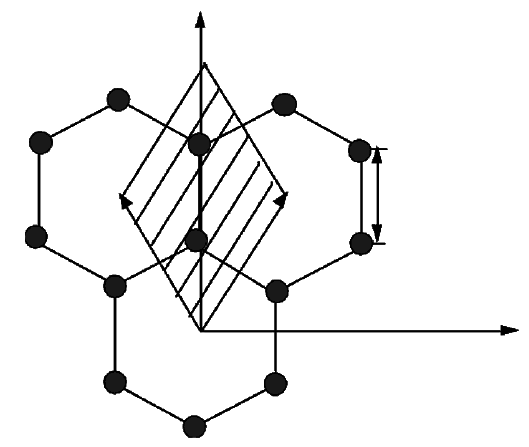
\includegraphics[width=0.5\textwidth]{pic/六方复式格子.png}
    \caption{六方复式格子}
    \label{fig:7.1}
\end{figure}

设 $\vec{a}_3=\vec{k}$,由图可得:

\begin{equation*}
    \vec{a}_1 = \frac{\sqrt{3}}{2} a \vec{i} + \frac{3}{2} a \vec{j}, \quad \vec{a}_2 = -\frac{\sqrt{3}}{2} a \vec{i} + \frac{3}{2} a \vec{j}
\end{equation*}

则原胞面积

\begin{equation*}
    A_c = \Omega = \vec{a}_3 \cdot (\vec{a}_1 \times\vec{a}_2) = \frac{3\sqrt{3}}{2} a^2
\end{equation*}

\begin{align*}
    \vec{b}_1 &= \frac{2\pi (\vec{a}_2 \times \vec{a}_3)}{\Omega} = \frac{2\pi}{a} \left(\frac{\sqrt{3}}{3}\vec{i} + \frac{1}{3}\vec{j}\right) \\
    \vec{b}_2 &= \frac{2\pi (\vec{a}_3 \times \vec{a}_1)}{\Omega} = \frac{2\pi}{a} \left(-\frac{\sqrt{3}}{3}\vec{i} + \frac{1}{3}\vec{j}\right) \\
    \vec{k}_h = \vec{b}_1 + \vec{b}_2 = \frac{4\pi}{3a} \vec{j}
\end{align*}

原胞中两个原子相对于原胞顶点的位矢分别为:

\begin{align*}
    \vec{d}_1 &= \frac{1}{3} \vec{a}_1 + \frac{1}{3} \vec{a}_2 = a \vec{j} \\
    \vec{d}_2 &= \frac{2}{3} \vec{a}_1 + \frac{2}{3} \vec{a}_2 = 2a \vec{j}
\end{align*}

晶体的结构因子为

\begin{equation*}
    S(\vec{k}_h) = \sum_{j=1}^{2} e^{-i \vec{k}_h \cdot \vec{d}_j} = e^{-i \frac{4\pi}{3a}\vec{j} \cdot a\vec{j}} + e^{-i \frac{4\pi}{3a}\vec{j} \cdot 2a\vec{j}} = -1
\end{equation*}

\noindent \textbf{6.\quad} 用紧束缚方法处理面心立方晶体的 $s$ 态电子,若只计最近邻的相互作用,试导出其能带为:

\begin{equation*}
    E(\vec{k}) = E_0 - A - 4J \left[\cos{\frac{k_x a}{2}}\cos{\frac{k_y a}{2}} + \cos{\frac{k_y a}{2}}\cos{\frac{k_z a}{2}} + \cos{\frac{k_z a}{2}}\cos{\frac{k_x a}{2}}\right]
\end{equation*}

并求能带底部电子的有效质量。

\noindent \textbf{解:}

面心立方的每个格点有 $12$ 个最近邻,如晶格常数为 $a$,取某格点为坐标原点,则这 $12$ 个最近邻的坐标为:

\begin{equation*}
    \begin{matrix}
        (\frac{a}{2}, -\frac{a}{2}, 0) & (\frac{a}{2}, \frac{a}{2}, 0) & (-\frac{a}{2}, \frac{a}{2}, 0) & (-\frac{a}{2}, -\frac{a}{2}, 0) \\
        (0, -\frac{a}{2}, -\frac{a}{2}) & (0, \frac{a}{2}, -\frac{a}{2}) & (0, \frac{a}{2}, \frac{a}{2}) & (0, -\frac{a}{2}, \frac{a}{2}) \\
        (\frac{a}{2}, 0, -\frac{a}{2}) & (\frac{a}{2}, 0, \frac{a}{2}) & (-\frac{a}{2}, 0, \frac{a}{2}) & (-\frac{a}{2}, 0, -\frac{a}{2})
    \end{matrix}
\end{equation*}

\begin{align*}
    E(\vec{k}) &= E^s + C - J \bigg[e^{i\vec{k}\cdot\left(\frac{a}{2}\vec{i}-\frac{a}{2}\vec{j}\right)} + e^{i\vec{k}\cdot\left(\frac{a}{2}\vec{i}+\frac{a}{2}\vec{j}\right)} + e^{i\vec{k}\cdot\left(-\frac{a}{2}\vec{i}+\frac{a}{2}\vec{j}\right)} + e^{i\vec{k}\cdot\left(-\frac{a}{2}\vec{i}-\frac{a}{2}\vec{j}\right)} \\
    &\quad\quad\quad\quad\quad\quad\quad e^{i\vec{k}\cdot\left(\frac{a}{2}\vec{j}-\frac{a}{2}\vec{k}\right)} + e^{i\vec{k}\cdot\left(\frac{a}{2}\vec{j}+\frac{a}{2}\vec{k}\right)} + e^{i\vec{k}\cdot\left(-\frac{a}{2}\vec{j}+\frac{a}{2}\vec{k}\right)} + e^{i\vec{k}\cdot\left(-\frac{a}{2}\vec{i}-\frac{a}{2}\vec{j}\right)} \\
    &\quad\quad\quad\quad\quad\quad\quad e^{i\vec{k}\cdot\left(\frac{a}{2}\vec{i}-\frac{a}{2}\vec{k}\right)} + e^{i\vec{k}\cdot\left(\frac{a}{2}\vec{i}+\frac{a}{2}\vec{k}\right)} + e^{i\vec{k}\cdot\left(-\frac{a}{2}\vec{i}+\frac{a}{2}\vec{k}\right)} + e^{i\vec{k}\cdot\left(-\frac{a}{2}\vec{i}-\frac{a}{2}\vec{k}\right)}\bigg] \\
    &= E^s + C - 4J \left[\cos{\frac{k_x a}{2}}\cos{\frac{k_y a}{2}} + \cos{\frac{k_y a}{2}}\cos{\frac{k_z a}{2}} + \cos{\frac{k_z a}{2}}\cos{\frac{k_x a}{2}}\right]
\end{align*}

对于上式表示的能带,其最小值位于倒空间的原点

\begin{equation*}
    E_{min} = E^s + C - 12J
\end{equation*}

令 $E_0 = E_{min}, A=-12J$,则有

\begin{equation*}
    E(\vec{k}) = E_0 - A - 4J \left[\cos{\frac{k_x a}{2}}\cos{\frac{k_y a}{2}} + \cos{\frac{k_y a}{2}}\cos{\frac{k_z a}{2}} + \cos{\frac{k_z a}{2}}\cos{\frac{k_x a}{2}}\right]
\end{equation*}

将上式中三角函数在 $k=0$ 附近展开,可得:

\begin{align*}
    E(\vec{k}) &= E_{min} + J a^2 (k_x^2+k_y^2+k_z^2) \\
    &= E_{min} + \frac{\hbar^2 k^2}{2 m^*}
\end{align*}

比较可得

\begin{equation*}
    m^* = \frac{\hbar^2}{2J a^2} > 0
\end{equation*}

\noindent \textbf{7.\quad} 二维正方晶格的周期性势场可表示为:

\begin{equation*}
    V(x, y) = -4U \cos\left(\frac{2\pi}{a}x\right) \cos\left(\frac{2\pi}{a}y\right)
\end{equation*}

$a$ 为晶格常数,试由自由电子近似计算布里渊区边界点 $(\frac{\pi}{a}, \frac{\pi}{a})$ 处的能隙。

\noindent \textbf{解:}

\begin{align*}
    V(x, y) &= \sum_{m, n} V_{mn} e^{im\frac{2\pi}{a}x} e^{in\frac{2\pi}{a}y} \\
    &= V_{00} + \sum_{m\ne 0, n\ne 0} V_{mn} e^{im\frac{2\pi}{a}x} e^{in\frac{2\pi}{a}y} \\
\end{align*}

为简单计算,令 $V_{00}=0$

\begin{equation*}
    V_{mn} = \frac{1}{a^2} \int_{-\frac{a}{2}}^{\frac{a}{2}} \int_{-\frac{a}{2}}^{\frac{a}{2}} V(x, y) e^{-im\frac{2\pi}{a}x} e^{-in\frac{2\pi}{a}y} \dif x \dif y
\end{equation*}

在边界点 $\left(\frac{\pi}{a}, \frac{\pi}{a}\right)$ 处,$m=n=1$

\begin{align*}
    V_{11} &= \frac{1}{a^2} \int_{-\frac{a}{2}}^{\frac{a}{2}} \int_{-\frac{a}{2}}^{\frac{a}{2}} V(x, y) e^{-i\frac{2\pi}{a}x} e^{-i\frac{2\pi}{a}y} \dif x \dif y \\
    &= \frac{1}{a^2} \int_{-\frac{a}{2}}^{\frac{a}{2}} \int_{-\frac{a}{2}}^{\frac{a}{2}} V(x, y) \cos{\frac{2\pi}{a}x} \cos{\frac{2\pi}{a}y} \dif x \dif y \\
    &= \frac{-4U}{a^2} \left[\int_{-\frac{a}{2}}^{\frac{a}{2}} \cos^2{\frac{2\pi}{a}x}\right]^2 \\
    &= \frac{-4U}{a^2} \left(\frac{a}{2}\right)^2 \\
    &= -U
\end{align*}

所以,在边界点 $\left(\frac{\pi}{a}, \frac{\pi}{a}\right)$ 处的能隙为

\begin{equation*}
    2|V_{11}| = 2U
\end{equation*}

\noindent \textbf{8.\quad} 图为二维正三角形晶格,相邻原子间距为 $a$, 只计入最近邻相互作用,试用紧束缚近似计算其 $s$ 电子能带 $\Delta E$、带中电子的速度 $v(k)$ 以及能带极值附近的有效质量 $m^*$。

\begin{figure}[htbp]
    \centering
    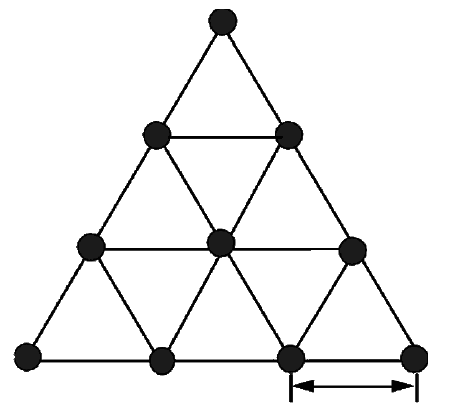
\includegraphics{pic/二维正三角晶格.png}
    \caption{二维正三角晶格}
    \label{fig:7.2}
\end{figure}

\noindent \textbf{解:}

三角形晶格的每个格点有 $6$ 个最近邻,晶格常数为 $a$,取某格点为坐标原点,则这 $6$ 个最近邻的坐标为:

\begin{equation*}
    (a, 0), \quad (\frac{a}{2}, \frac{\sqrt{3}}{2}a), \quad (-\frac{a}{2}, \frac{\sqrt{3}}{2}a), \quad (-a, 0), \quad (-\frac{a}{2}, \frac{\sqrt{3}}{2}a), \quad (\frac{a}{2}, -\frac{\sqrt{3}}{2}a)
\end{equation*}

\begin{align*}
    E(\vec{k}) &= E^s + C - J \sum_l e^{i\vec{k}\cdot\vec{R}_l} \\
    &= E^s + C - J \left[e^{i\vec{k}\cdot a\vec{i}} + e^{i\vec{k}\cdot \left(\frac{a}{2}\vec{i}+\frac{\sqrt{3}}{2}a\vec{j}\right)} + e^{i\vec{k}\cdot \left(-\frac{a}{2}\vec{i}+\frac{\sqrt{3}}{2}a\vec{j}\right)} + e^{i\vec{k}\cdot (-a\vec{i})} + e^{i\vec{k}\cdot \left(-\frac{a}{2}\vec{i}-\frac{\sqrt{3}}{2}a\vec{j}\right)} + e^{i\vec{k}\cdot \left(\frac{a}{2}\vec{i}-\frac{\sqrt{3}}{2}a\vec{j}\right)}\right] e^{i\vec{k}\cdot\vec{R}_l} \\
    &= E^s + C - J \left(2\cos{k_x a} + 4\cos{\frac{k_x a}{2}} \cos{\frac{\sqrt{3}k_y a}{2}}\right)
\end{align*}

\begin{align*}
    E(\vec{k}) &= \frac{1}{\hbar} \Delta_k(\vec{k}) \\
    &= \frac{2Ja}{\hbar} \left[\left(\sin{k_x a} + \sin{\frac{k_x a}{2}} \cos{\frac{\sqrt{3}k_y a}{2}}\right) \vec{e}_x + \left(\sqrt{3} \cos{\frac{k_x a}{2}} \sin{\frac{\sqrt{3}k_y a}{2}}\right) \vec{e}_y\right]
\end{align*}

倒空间的原点 $(0, 0)$ 处,能带的极小值为

\begin{equation*}
    E_{min} = E^s + C - 6J
\end{equation*}

倒空间 $(\frac{4\pi}{3a}, 0)$ 或 $(\frac{2\pi}{3a}, \frac{2\pi}{\sqrt{3}a})$ 处,能带的极大值为

\begin{equation*}
    E_{max} = E^s + C + 3J
\end{equation*}

所以能带大小为

\begin{equation*}
    \Delta E = 9J
\end{equation*}

在能带极小值,将 $E(\vec{k})$ 中的三角函数在 $\vec{k}=0$ 附近用泰勒级数展开可得:

\begin{equation*}
    E(\vec{k}) = E_{min} + \frac{3}{2} J a^2 (k_x^2 + k_y^2) = E_{min} + \frac{\hbar^2 k^2}{2 m^*}
\end{equation*}

比较可得

\begin{equation*}
    m^* = \frac{\hbar^2}{3J a^2}
\end{equation*}

在能带极大值,如 $(\frac{4\pi}{3a}, 0)$ 附近将 $E(\vec{k})$ 中的三角函数用泰勒级数展开,令 $k_x=\frac{4\pi}{3a}+\delta k_x, k_y=\delta k_y$,可得

\begin{equation*}
    E(\vec{k}) = E_{max} - \frac{3}{4}J a^2 \left[(\delta k_x)^2 + (\delta k_y)^2\right] = E_{min} + \frac{\hbar2 (\delta k)^2}{2 m^*}
\end{equation*}

比较可得

\begin{equation*}
    m^* = -\frac{2\hbar^2}{3J a^2} < 0
\end{equation*}

